\chapter{初中代数总复习参考题\footnotemark}\label{app:1}
\footnotetext{这是供复习初中代数时参考选用的习题。}

\begin{xiaotis}
\begin{enhancedline}

\xiaoti{列出实数的分类表。}

\xiaoti{计算:}
\begin{xiaoxiaotis}

    \xxt{$4 \times 0.2^2 - 10 \times 1.1^3 + 3 \times \sqrt{5.14} - \sqrt[3]{5.26}$ (保留三个有效数字);}

    \xxt{$3a^3 - [-5a^2 + a(-4a^2 + 2a - 1) + 4] - 7$ (精确到 $0.01$),其中 $a = 2.35$。}

\end{xiaoxiaotis}


\xiaoti{}%
\begin{xiaoxiaotis}%
    \xxt[\xxtsep]{若 $(a - 1)^2 + (b + 2)^2 = 0$, $a$、$b$ 为实数,求 $a$、$b$;}

    \xxt{若 $x^2 + 2x + y^2 - 6y + 10 = 0$, $x$、$y$ 为实数,求 $x$、$y$。}

\end{xiaoxiaotis}


\xiaoti{计算下列各题:}
\begin{xiaoxiaotis}

    \xxt{$(a^3 - a^2b + ab^2 - b^3)(a + b)$;}

    \xxt{$(a + b)^2 (a - b)^2 - (a^2 + b^2) (a^2 - b^2)$;}

    \xxt{$(p + q - m - n) (p - q - m + n)$;}

    \xxt{$(x + 2y - z) (x - 2y + z) - (x + 2y + z)^2$;}

    \xxt{$(x^5 + x^4 + x^3 + x^2 + x + 1) \div (x + 1)$;}

    \xxt{$(x^4 + x^2 + 1) \div (x^2 - x + 1)$。}

\end{xiaoxiaotis}


\xiaoti{}%
\begin{xiaoxiaotis}%
    \xxt[\xxtsep]{已知 $x^2 + x - 1 = 0$,求 $x^3 + 2x^2 + 3$ 的值;}

    \xxt{若 $bc = ad$,求证: $ab(c^2 - d^2) = (a^2 - b^2)cd$;}

    \xxt{若 $a + b + c = 0$,求证:$a^3 + a^2c + b^2c - abc + b^3 = 0$;}

    \xxt{证明:$a^2(b - c) + b^2(c - a) + c^2(a - b) = -(a - b) (b - c) (c - a)$。}

\end{xiaoxiaotis}


\xiaoti{分解因式:}
\begin{xiaoxiaotis}

    \begin{tblr}{columns={18em, colsep=0pt}}
        \xxt{$x^5 - x^4 + x^3 - x^2 + x - 1$;}    & \xxt{$3x^2 - 2x - 8$;} \\
        \xxt{$4x^2 + 2x + \exdfrac{1}{4} - y^2$;} & \xxt{$l^4 - 3\,l^2 + 1$;} \\
        \xxt{$a^2 - 2ab + b^2 - 6a + 6b + 5$;}    & \xxt{$(1 - a^2) (1 - b^2) - 4ab$。}
    \end{tblr}
\end{xiaoxiaotis}


\xiaoti{在实数集合内分解因式:}
\begin{xiaoxiaotis}

    \begin{tblr}{columns={18em, colsep=0pt}}
        \xxt{$x^2 + x - 1$;}     & \xxt{$x^4 + x^2 - 6$;} \\
        \xxt{$6x^4 - 7x^2 - 3$;} & \xxt{$x^4 + 3x^3 + x^2$。}
    \end{tblr}
\end{xiaoxiaotis}


\xiaoti{$x$ 取什么值时,代数式 $\dfrac{-(x - 5)}{(3 - x) (x + 1)}$ 的值满足下列条件?}
\begin{xiaoxiaotis}

    \begin{tblr}{columns={12em, colsep=0pt}}
        \xxt{等于 $0$;} & \xxt{没意义;} & \xxt{等于 $1$。}
    \end{tblr}
\end{xiaoxiaotis}


\xiaoti{计算下列各题:}
\begin{xiaoxiaotis}

    \xxt{$\dfrac{x^2 + 2x + 1}{x^3 - x} \cdot \dfrac{x}{x + 1} - \dfrac{1}{x + 1}$;}

    \xxt{$\dfrac{1}{1 - x} + \dfrac{1}{1 + x} + \dfrac{2}{1 + x^2} + \dfrac{4}{1 + x^4}$;}

    \xxt{$\dfrac{x + 2}{x + 1} - \dfrac{x + 3}{x + 2} + \dfrac{x + 4}{x + 3} - \dfrac{x + 5}{x + 4}$;}

    \xxt{$\dfrac{a^2}{(a - b) (a - c)} + \dfrac{b^2}{(b - a) (b - c)} + \dfrac{c^2}{(c - a) (c - b)}$。}

\end{xiaoxiaotis}



\xiaoti{试证下列各题:}
\begin{xiaoxiaotis}

    \xxt{若 $\exdfrac{a}{b} + \exdfrac{b}{a} = x$,  $\exdfrac{a}{b} - \exdfrac{b}{a} = y$。求证: $x^2 - y^2 = 4$;}

    \xxt{若 $a$、$b$、$c$ 为实数,且 $a^2 + b^2 + c^2 - ab - bc - ca = 0$。求证 $a = b = c$。}

\end{xiaoxiaotis}


\xiaoti{计算:}
\begin{xiaoxiaotis}

    \xxt{$5\sqrt{28} + 3\sqrt{63} - 10\sqrt{7} + 3\sqrt{\exdfrac{1}{7}}$;}

    \xxt{$4\sqrt[6]{125} - 3\sqrt[4]{25} + \sqrt{\exdfrac{4}{5}}$;}

    \xxt{$(2\sqrt{3} + \sqrt{6}) (\sqrt{3} - 2\sqrt{6})$;}

    \xxt{$\sqrt{(\sqrt{2} - \sqrt{3})^2} + \sqrt{(\sqrt{3} - \sqrt{2})^2}$;}

    \xxt{$\sqrt{xy} \left( \sqrt{xy} - 3\sqrt{\exdfrac{y}{x}}  - 2\sqrt{\exdfrac{x}{y}} + 4\sqrt{\dfrac{1}{xy}} \right) \; (x > 0,\; y > 0)$;}

    \xxt{$\dfrac{1}{1 - \sqrt[4]{x}} + \dfrac{1}{1 + \sqrt[4]{x}} + \dfrac{2}{1 + \sqrt{x}} + \dfrac{4}{1 + x}$。}

\end{xiaoxiaotis}


\xiaoti{化简 $\sqrt{\dfrac{x^2 - 6x + 9}{x^2 + 6x + 9}}$。}

\xiaoti{解下列方程:}
\begin{xiaoxiaotis}

    \xxt{$\dfrac{2 - x}{6} - \dfrac{2x - 3}{4} = 1$;}

    \xxt{$\dfrac{3x + 6}{8} - \left( \dfrac{5x}{6} - 1 \right) = \exdfrac{5}{6}$;}

    \xxt{$\exdfrac{1}{3} \left( 3x - \dfrac{10 - 7x}{2} \right) - \exdfrac{1}{6} \left( 2x - \dfrac{2x + 2}{3} \right) = \exdfrac{x}{2} - 1$;}

    \xxt{$\exdfrac{1}{3}(x - 2) - \exdfrac{1}{7}(5x - 6) = \dfrac{22x - 63}{105} - \exdfrac{1}{5}(3x - 4)$;}

    \xxt{$\dfrac{ax}{b} + \dfrac{bx}{a} - 1 = 0$;($a$,$b$ 为已知数)}

    \xxt{$\dfrac{mx + 1}{n} + \dfrac{nx + 1}{m} = 1$。($m$,$n$ 为已知数)}

\end{xiaoxiaotis}


\xiaoti{解下列方程组:}
\begin{xiaoxiaotis}

    \xxt{$\begin{cases}
        \exdfrac{1}{2}(x + 11) = \exdfrac{1}{3}(y + 13) + 2 \douhao \\
        5x = 3y + 8 \fenhao
    \end{cases}$}

    \xxt{$\begin{cases}
        \dfrac{2x}{3} + \dfrac{3y}{4} = \dfrac{3x - 2y}{2} + 1 \douhao \\[1em]
        \dfrac{3x}{2} - \dfrac{4y}{3} = \dfrac{3x + 4y}{6} - 1 \fenhao
    \end{cases}$}

    \xxt{$\begin{cases}
        \dfrac{3}{x - 4} + \dfrac{4}{y - 1} = 3 \douhao \\[1em]
        \dfrac{9}{x - 4} - \dfrac{2}{y - 1} = 2 \fenhao
    \end{cases}$}

    \xxt{$\dfrac{2x + y + 6}{4} = \dfrac{4x - 3y - 7}{6} = \dfrac{-6x - 7y + 10}{8}$;}

    \xxt{$\begin{cases}
        2x + 3y - 4z = 4 \douhao \\[0.5em]
        2y + 3z = \dfrac{17}{12} \douhao \\[1em]
        x + 4y = \dfrac{10}{3} \fenhao
    \end{cases}$}

    \xxt{$\begin{cases}
        x + y - z = 3 \douhao \\
        z + x - y = 1 \douhao \\
        y + z - x = 7 \juhao
    \end{cases}$}

\end{xiaoxiaotis}


\xiaoti{解方程:}
\begin{xiaoxiaotis}

    \xxt{$4(x + 3)^2 - 9(x - 2)^2 = 0$;}

    \xxt{$\sqrt{3}(y^2 - y) = \sqrt{2}(y^2 - y)$;}

    \xxt{$x^2 - (2 - 2\sqrt{2})x + 3 - 2\sqrt{2} = 0$;}

    \xxt{$(t + 6) (t - 6) = 2(t - 3)$;}

    \xxt{$(x + 2)^2 + (x - 1)^2 = x^2 + 6$;}

    \xxt{$2(x + 5) (x - 5) = (x - 6)^2$。}

\end{xiaoxiaotis}


\xiaoti{已知二次方程 $x^2 - mx + 2m = 0$ 的一个根是 $1$,}%
\begin{xiaoxiaotis}%
    \xxt[\xxtsep]{求 $m$ 的值;}
    \xxt[\xxtsep]{求另一个根。}

\end{xiaoxiaotis}


\xiaoti{不解方程,求方程 $2x^2 - 7x + 2 = 0$ 的两根的倒数的和。}


\xiaoti{}%
\begin{xiaoxiaotis}%
    \xxt[\xxtsep]{解分式方程和根式方程时,为什么验根是必要的步骤?}

    \xxt{解下列方程:}

    % 由于仅本题才有这种情况,所以就手工写编号。
    \hspace{4em} \tc{1} $\dfrac{x- 1}{x^2 - 2x} + \dfrac{x - 2}{x^2 - x} - \dfrac{x}{x^2 - 3x + 2} = 0$;

    \hspace{4em} \tc{2} $\left( \dfrac{x^2 - 1}{x} \right)^2 + \exdfrac{7}{6} \left( \dfrac{x^2 - 1}{x} \right) - 4 = 0$;

    \hspace{4em} \tc{3} $x^2 + 3x - \dfrac{20}{x^2 + 3x} = 8$;

    \hspace{4em} \tc{4} $\sqrt{5x +4} - \sqrt{2x - 1} - \sqrt{3x + 1} = 0$;

    \hspace{4em} \tc{5} $x^2 + 3x - 2\sqrt{x^2 + 3x - 1} - 4 = 0$;

    \hspace{4em} \tc{6} $x^4 - 25x^2 + 144 = 0$;

    \hspace{4em} \tc{7} $(x^2 + 5x)^2 - 2x^2 - 10x - 24 = 0$;

    \hspace{4em} \tc{8} $(x^2 + 5x - 12) (x^2 + 5x + 2) = 32$。

\end{xiaoxiaotis}


\xiaoti{解下列方程组:}
\begin{xiaoxiaotis}

    \xxt{$\begin{cases}
        (x + y)^2 - 3(x + y) = 54 \douhao \\
        (x - y)^2 - 5(x - y) = 14 \fenhao
    \end{cases}$}

    \xxt{$\begin{cases}
        a + aq^2 = 15 \douhao \\
        aq + aq^3 = 30 \fenhao
    \end{cases}$}

    \xxt{$\begin{cases}
        \dfrac{3x - 5y}{2xy} = \exdfrac{4}{3} \douhao \\[1em]
        \exdfrac{3}{x} + \exdfrac{1}{y} = 4 \fenhao
    \end{cases}$}

    \xxt{$\begin{cases}
        \sqrt{\exdfrac{x}{y}} + \sqrt{\exdfrac{y}{x}} = \exdfrac{5}{2} \douhao \\
        x + y = 5 \fenhao
    \end{cases}$}

    \xxt{$\begin{cases}
        x + xy + y = 11 \douhao \\
        x^2y + xy^2 = 30 \juhao
    \end{cases}$}

\end{xiaoxiaotis}


\xiaoti{}%
\begin{xiaoxiaotis}%
    \xxt[\xxtsep]{从 $\begin{cases}
        mu = s(m - 1) \douhao \\
        f = s - u \douhao
    \end{cases}$ (这里 $m \neq 0$) 导出 $f$、$s$、$m$ 间的一个关系式;}

    \xxt{从 $\begin{cases}
        I_k = I_a + I_c \douhao \\
        I_c = mI_k \douhao
    \end{cases}$ (这里 $m \neq 1$) 导出 $I_c$、$m$、$I_a$ 间的一个关系式。}

\end{xiaoxiaotis}


\renewcommand{\lfm}{\mathord{\text{m}^3}}%立方米
\xiaoti{甲贮水池内有水 $380 \; \lfm$, 乙贮水池内有水 $1500 \; \lfm$。
    甲贮水池每小时进水 $80 \; \lfm$, 乙贮水池每小时抽出水 $60 \; \lfm$。
    经过几小时,两个贮水池内的水一样多?
}


\xiaoti{甲、乙二人在 $400$ 米长的环形跑道上练习自行车,甲的速度比乙的速度快。
    当他们都从某处同时出发背向行驶时,每隔 $40$ 秒就相遇一次,同向行驶时,
    隔 $6$ 分 $40$ 秒相遇一次。求甲,乙两人骑车的速度。
}


\xiaoti{某项工作,甲、乙两人合作,$16$ 天可以完成。如果共同做了 $4$ 天后,
    剩余工作由乙单独完成,需要的时间比由甲一人完成全部工作的时间多 $12$ 天。
    问单独完成全部工作,甲、乙各需要多少天?
}

\begin{minipage}{9cm}
    \xiaoti{如图,一块长 $25$ 厘米,宽 $18$ 厘米的铁板,在去掉一个与三边相切的圆后,
        剩下的铁板能剪出的最大圆的直径是多少?
    }

    \xiaoti{某车间每天能生产甲种零件 $500$ 只,或者乙种零件 $600$ 只,或者丙种零件 $750$ 只。
        甲、乙、丙三种零件各一只配成一套。现在要在 $30$ 天内生产最多的成套产品,
        甲、乙、丙三种零件各应生产多少天?
    }
\end{minipage}
\quad
\begin{minipage}{6cm}
    \begin{figure}[H]
        \centering
        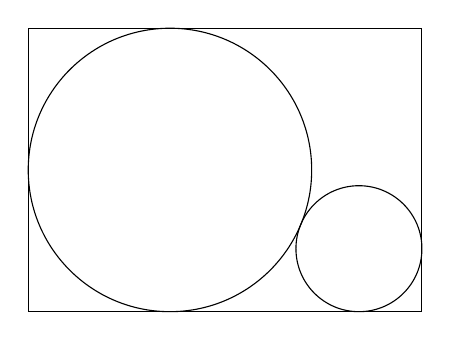
\begin{tikzpicture}
    \pgfmathsetmacro{\factor}{0.2}
    \pgfmathsetmacro{\a}{25 * \factor}% 长
    \pgfmathsetmacro{\b}{18 * \factor}% 宽

    \pgfmathsetmacro{\R}{\b/2}

    % 以长方形左下角的点为坐标原点,设大、小圆半径分别为 R、r。则:
    % 大圆圆心 A 点坐标  (R, R)
    % 小圆圆心 B 点坐标  (a - r, r)
    % 两圆相切,所以 AB 的距离 = R + r。
    % 代入两点的距离公式得
    %       sqrt{[R - (a - r)]^2 + (R - r)^2} = R + r
    % 化简后得
    %       r = (R + a) - \sqrt(4aR)
    \pgfmathsetmacro{\r}{\R + \a - sqrt(4 * \a * \R)}

    \coordinate (A) at (\R, \R);
    \coordinate (B) at (\a - \r, \r);

    \draw (0, 0) rectangle (\a, \b);
    \draw (A) circle (\R);
    \draw (B) circle (\r);
\end{tikzpicture}


        \caption*{(第 24 题)}
    \end{figure}
\end{minipage}


\xiaoti{一种灭虫药粉 $40$ 公斤,含药率是 $15\%$,现在要用含药率较高的同样的灭虫药粉 $50$ 千克和它混合,
    使混合后的含药率在 $25\%$ 与 $30\%$ 之间(不包括 $25\%$ 和 $30\%$),求所用的药粉的含药率。
}


\xiaoti{解下列不等式或不等式组,并把它们的解集在数轴上表示出来:}
\begin{xiaoxiaotis}

    \xxt{$2(x + 1) + \dfrac{x - 2}{3} > \dfrac{7x}{2} - 1$;}

    \xxt{$2x - \dfrac{x - 1}{2} < \dfrac{2x - 1}{3} + \dfrac{x + 1}{6}$;}

    \xxt{$\exdfrac{1}{2} \{1 - 2[x - 4(x - 1)]\} \leqslant 4x$;}

    \xxt{$-1 \leqslant \dfrac{3 - x}{2} \leqslant 2$;}

    \xxt{$-4 \leqslant \dfrac{3x - 5}{2} \leqslant -2$;}

    \xxt{$\begin{cases}
        3x - 5 \geqslant 2x + 3 \douhao \\
        \dfrac{x - 5}{2} \leqslant 3x + 1 \juhao
    \end{cases}$}

\end{xiaoxiaotis}


\xiaoti{在数轴上表示适合下列条件的数的集合:}
\begin{xiaoxiaotis}

    \xxt{使不等式 $x \leqslant 5$ 或 $x > -2$ 成立;}

    \xxt{使不等式 $x \leqslant 5$ 与 $x > -2$ 同时成立;}

    \xxt{使不等式 $x > 5$ 或 $x > -2$ 成立;}

    \xxt{使不等式 $x > 5$ 与 $x > -2$ 同时成立;}

    \xxt{使不等式 $x > 5$ 或 $x \leqslant -2$ 成立;}

    \xxt{使不等式 $x > 5$ 与 $x \leqslant -2$ 同时成立。}

\end{xiaoxiaotis}


\xiaoti{计算:}
\begin{xiaoxiaotis}

    \xxt{$(-3x^{\frac{1}{3}} y^{\frac{1}{4}}) (2x^{-\frac{2}{3}} y^{-\frac{1}{2}}) (-x^{-\frac{2}{3}} y^{\frac{1}{4}})$;}

    \xxt{$\left( \dfrac{m^4 n^{-4}}{m^{-1} n} \right)^{-3} \div \left( \dfrac{m^{-2} n^2}{m n^{-1}}\right)^5$;}

    \xxt{$(3x^{\frac{1}{2}} - 2y^{-\frac{1}{2}}) (3x^{\frac{1}{2}} + 2y^{-\frac{1}{2}})$;}

    \xxt{$\sqrt[3]{3} \cdot \sqrt[4]{4} \cdot \sqrt[6]{6}$;}

    \xxt{$\sqrt[\uproot{6}3]{x^{-5} y^2 \sqrt{x^3 y}}$;}

    % 用了两种不同的方法,将 \sqrt[4]{y} 的根号向上移,尽量与之前的 \sqrt{2x} 的根号平齐。
    \xxt{$(\sqrt{2x} - 3\sqrt[4]{\smash[b]{y}}) (\sqrt{2x} + 3\sqrt[4]{\rule{0pt}{1.65ex} y})$。}

\end{xiaoxiaotis}


\xiaoti{}%
\begin{xiaoxiaotis}%
    \xxt[\xxtsep]{为什么利用对数可以用加法计算乘法,用减法计算除法?}

    \xxt{用科学记数法写出下列各数,并说明它们的常用对数的首数:\\
        \hspace*{2em} $54890 \fenhao \quad 0.08351 \fenhao \quad 4.309 \fenhao \quad 213.7 \juhao$
    }

\end{xiaoxiaotis}


\xiaoti{已知 $\lg 2 = 0.3010$, 试判定 $2^7 \times 8^{11} \times 5^{11}$ 是几位数。}


\xiaoti{利用对数计算:}

\begin{xiaoxiaotis}

    \begin{tblr}{columns={18em, colsep=0pt}}
        \xxt{$\sqrt[\uproot{6}8]{\dfrac{0.3586 \times \sqrt[4]{257}}{0.00501}}$;}
            & \xxt{$\dfrac{32.85^2 - 12.64^2}{32.85 \times 12.64} \div \sqrt{\dfrac{32.85}{12.64}}$。}
    \end{tblr}
\end{xiaoxiaotis}


\xiaoti{求下列函数的自变量的取值范围:}

\begin{xiaoxiaotis}

    \begin{tblr}{columns={18em, colsep=0pt}}
        \xxt{$y = \dfrac{x - 5}{x^2 - 3x + 2}$;} & \xxt{$y = \sqrt{8 - 2x - x^2}$。}
    \end{tblr}
\end{xiaoxiaotis}


%(编号在题干上,无法处理,所以手工写编号)
\xiaoti{已知 $y_1 = 2x - 3$, $y_2 = -3x + 7$, 计算 $x$ 取何值时,\\
    \begin{tblr}{columns={12em, colsep=0pt}, rows={rowsep=0pt}}
        (1)$y_1 > y_2$; & (2)$y_1 = y_2$; & (3)$y_1 < y_2$。
    \end{tblr} \\
    并用图象加以说明。
}


\xiaoti{计算 $k$ 为何值时 $y = -x^2 + 2x + k$ 的图象与 $x$ 轴 \\
    \begin{tblr}{columns={12em, colsep=0pt}, rows={rowsep=0pt}}
        (1)相交于一点; & (2)相交于两点; & (3)不相交。
    \end{tblr} \\
    并用图象加以说明。
}


\xiaoti{函数 $y = x^2 + px + q$ 的最小值是 $4$。 在 $x = 2$ 时,$y = 5$。求 $p$、$q$ 的值。}


\xiaoti{设 $\alpha$ 是 $0^\circ$ ~ $180^\circ$ 间的角。根据下列条件求 $\alpha$。
    如果有解,求出所有的解:
}
\begin{xiaoxiaotis}

    \begin{tblr}{columns={12em, colsep=0pt}}
        \xxt{$\tan\alpha = -1$;}       & \xxt{$\cos\alpha = 0$;}               & \xxt{$\sin\alpha = \exdfrac{1}{2}$;} \\
        \xxt{$\cot\alpha = \sqrt{3}$;} & \xxt{$\sin\alpha = -\exdfrac{1}{2}$;} & \xxt{$\cos\alpha = \sqrt{2}$。}
    \end{tblr}
\end{xiaoxiaotis}


\xiaoti{在直角三角形 $ABC$ 中,斜边 $AB$ 上的高 $CD = 21$ cm, $AD = 18$ cm,
    解这个三角形(边长保留两个有效数字,角度精确到 $1^\circ$)。
}


\xiaoti{在半径为 $10.0$ cm 的圆中,作内接正五角星 $ABCDE$,
    求这五角星的顶点 $A$ 和 $B$ 间的距离,以及顶点 $A$ 和 $C$ 间的拒离(精确到 $0.1$ cm)。
}


\xiaoti{已知 $B = 30^\circ$, $c = 150$, $b = 50\sqrt{3}$,
    问满足条件的三角形 $ABC$ 有什么特点。
}


\xiaoti{求证:在 $\triangle ABC$ 中,如果 $\sin^2 A + \sin^2 B = \sin^2 C$,
    那么这个三角形一定是直角三角形。
}


\begin{minipage}{11cm}
    \xiaoti{如图,在小山顶上有一电视发射塔,塔高 $AB$ 是 $50$ 米,在平地上 $C$ 点,
        测得 $B$ 的仰角是 $40^\circ$, $A$ 的仰角是 $70^\circ$,
        求小山 $BD$ 的高(精确到 $1$ 米)。
    }

    \xiaoti{平行四边形 $ABCD$ 中,$AB = 8$, $AD = 5$, $\angle A = 60^\circ$,
        如果取 $A$ 作原点, $AB$ 所在的直线作 $x$ 轴,$C$ 点所在的象限作第一象限,
        求它的各个顶点的坐标。
    }


    \xiaoti{设 $l$ 是第一、第三象限内两坐标轴夹角的平分线,在 $l$ 上求一点,
        使它和两点 $A(8,\; 0)$、 $B(1,\; -3)$ 的距离相等。
    }

    \xiaoti{求证:$(-4,\; 3)$, $(8,\; 8)$, $(13,\; -4)$, $(1,\; -9)$ 是一个正方形的四个顶点。}
\end{minipage}
\quad
\begin{minipage}{4cm}
    \begin{figure}[H]
        \centering
        \begin{tikzpicture}[
    shan/.style={decorate, decoration={random steps,segment length=2pt,amplitude=1pt}},
]
    \pgfmathsetmacro{\factor}{0.05}
    \pgfmathsetmacro{\ab}{50 * \factor}
    \pgfmathsetmacro{\dcb}{40}
    \pgfmathsetmacro{\dca}{70}

    % 因为 cot(DCB) = CD/BD
    % 所以 CD = cot(DCB) * BD
    % 同理 CD = cot(DCA) * AD = cot(DCA) * (AB + BD)
    % 所以 cot(DCB) * BD = cot(DCA) * (AB + BD)
    % 化简后得:
    %      BD = [ cot(DCA) * AB ] / [ cot(DCB) - cot(DCA) ]
    \pgfmathsetmacro{\bd}{cot(\dca) * \ab / (cot(\dcb) - cot(\dca))}
    \pgfmathsetmacro{\cd}{cot(\dcb) * \bd}

    \coordinate ["$D$" below] (D) at (0, 0);
    \coordinate ["$C$" below] (C) at (-\cd, 0);
    \coordinate ["$B$" right] (B) at (0, \bd);
    \coordinate ["$A$" above] (A) at (0, \bd + \ab);

    \draw [thick] (-1.8, 0) -- (1.2, 0);
    \draw [thick] (C) -- (A);
    \draw [thick] (C) -- (B);
    \draw [dashed] (D) -- (B);

    \coordinate (B1) at ($(B) + (-0.2, 0)$);
    \coordinate (B2) at ($(B) + ( 0.2, 0)$);
    \draw [name path=b1] (A) -- (B1);
    \draw [name path=b2] (A) -- (B2);
    \foreach \y in {1, ..., 8} {
        \path [name path=xline] (-1, \bd + \ab*\y/9) -- (1, \bd + \ab*\y/9);
        \path [name intersections={of=b1 and xline, by=NB1}];
        \path [name intersections={of=b2 and xline, by=NB2}];
        \draw (B1) -- (NB2) -- (NB1) -- (B2);
        \coordinate (B1) at (NB1);
        \coordinate (B2) at (NB2);
    }

    \draw [shan] (-0.9, 0) to [out=30, in=180] (B);
    \draw [shan] (0.9, 0) to [out=150, in=0] (B);
\end{tikzpicture}


        \caption*{(第 42 题)}
    \end{figure}
\end{minipage}

\xiaoti{已知在 $n$ 个数据中,$x_1$ 出现 $f_1$ 次, $x_2$ 出现 $f_2$ 次,$\cdots$,
    $x_k$ 出现 $f_k$ 次 ($f_1 + f_2 + \cdots + f_k = n$),
    $\overline{x}$ 是这 $n$ 个数据的平均数。求证:
    $$ f_1(x_1 - \overline{x}) + f_2(x_2 - \overline{x}) + \cdots + f_k(x_k - \overline{x}) = 0 \juhao $$
}


\xiaoti{有甲、乙两种水稻,测得每种水稻各 $10$ 穴的分蘖数如下:\\
    \hspace*{4em}
    \begin{datatblr}{column{1}={mode=text}}
        甲: & 15 &  9 & 16 & 18 & 14 &  8 & 12 & 10 & 17 & 11 \\
        乙: & 12 & 15 & 14 & 16 & 15 & 13 & 12 & 10 & 12 & 10
    \end{datatblr} \\
    哪种水稻分蘖比较整齐?
}


\xiaoti{在生产过程中,测得维尼纶的纤度(表示纤维粗细的一种量)有如下的 $100$ 个数据,
    试列出样本的频率分布表和绘出频率分布直方图。\\
    \hspace*{4em}
    \begin{datatblr}{}
        1.36 & 1.49 & 1.43 & 1.41 & 1.37 & 1.40 & 1.32 & 1.42 & 1.47 & 1.39 \\
        1.41 & 1.36 & 1.40 & 1.34 & 1.42 & 1.42 & 1.45 & 1.35 & 1.42 & 1.39 \\
        1.44 & 1.42 & 1.39 & 1.42 & 1.42 & 1.30 & 1.34 & 1.42 & 1.37 & 1.36 \\
        1.37 & 1.34 & 1.37 & 1.37 & 1.44 & 1.45 & 1.32 & 1.48 & 1.40 & 1.45 \\
        1.39 & 1.46 & 1.39 & 1.53 & 1.36 & 1.48 & 1.40 & 1.39 & 1.38 & 1.40 \\
        1.36 & 1.45 & 1.50 & 1.43 & 1.38 & 1.43 & 1.41 & 1.48 & 1.39 & 1.45 \\
        1.37 & 1.37 & 1.39 & 1.45 & 1.31 & 1.41 & 1.44 & 1.44 & 1.42 & 1.47 \\
        1.35 & 1.36 & 1.39 & 1.40 & 1.38 & 1.35 & 1.42 & 1.43 & 1.42 & 1.42 \\
        1.42 & 1.40 & 1.41 & 1.37 & 1.46 & 1.36 & 1.37 & 1.27 & 1.37 & 1.38 \\
        1.42 & 1.34 & 1.43 & 1.42 & 1.41 & 1.41 & 1.44 & 1.48 & 1.55 & 1.37
    \end{datatblr}
}

\end{enhancedline}
\end{xiaotis}

